

%----------------------------------------------------------------------------------------
%	PACKAGES AND DOCUMENT CONFIGURATIONS
%----------------------------------------------------------------------------------------

\documentclass[a4paper,12pt]{article}
\usepackage[margin=1in]{geometry}
\renewcommand{\baselinestretch}{1.2}
\usepackage{siunitx} % Provides the \SI{}{} and \si{} command for typesetting SI units
\usepackage{graphicx} % Required for the inclusion of images
\usepackage{subfigure}
\usepackage{multirow}
\usepackage{amsmath} % Required for some math elements 
\usepackage{indentfirst}
\usepackage{times} % Uncomment to use the Times New Roman font
\usepackage{appendix}
\usepackage{float}  
\usepackage{verbatim}
\renewcommand{\multirowsetup}{\centering}  


%----------------------------------------------------------------------------------------
%	DOCUMENT INFORMATION
%----------------------------------------------------------------------------------------

\title{\rule{\textwidth}{0.3mm} \\UM–SJTU JOINT INSTITUTE \\ PHYSICS LABORATORY \\ (VP241) \\ \rule{\textwidth}{0.3mm} \\ [30 mm]  \Large{Laboratory Report} \\[5 mm]  Exercise 2 \\[1 mm] 
The Hall Probe: Characteristics and Applications \\[20 mm]} % Title
\author{Cao Zhiyuan} % Author name
\date{\today} % Date for the report

\begin{document}
\scshape

\maketitle % Insert the title, author and date

\begin{center}
\begin{tabular}{l l l}
\\[5 mm]
Partners:  \\
Name: Cao Zhiyuan & ID: 518370910030 & Group: 19 \\
~\\
Date Performed:\\
November 22, 2019\\
\end{tabular}
\end{center}

\thispagestyle{empty}


\newpage


\small\tableofcontents
\thispagestyle{empty}


\newpage

%----------------------------------------------------------------------------------------
%	SECTION 1
%----------------------------------------------------------------------------------------
\setcounter{page}{1}
\upshape
\section{\textsc{Objective}}
\begin{itemize}
\item Use Hall probe to understand the Hall effect.
\item Discover the practical applications of the principle of the Hall effect.
\item Verify the fact that the Hall voltage is proportional to the magnetic field.
\item Study the sensitivity of an integrated Hall probe.
\item Measure the magnetic field distribution along the axis of the solenoid and compare it with the theoretical value.
\end{itemize}

%----------------------------------------------------------------------------------------
%	SECTION 2
%----------------------------------------------------------------------------------------
\section{\textsc{Theoretical background}}
\subsection{\textsc{Hall Effect}}
Hall effect refers to the situation where a conducting sheet is placed in a magnetic field so that the plane of the sheet is perpendicular to the direction of the magnetic field B, and then if an electric current passes through the sheet in a particular direction, an electric potential difference will be generated between side a and b, which is shown in Fig.1. Such potential difference will result in a electric field and we define the corresponding potential difference as the Hall voltage, denoted as $U_H$.

\begin{figure}[htb] 
    \centering
    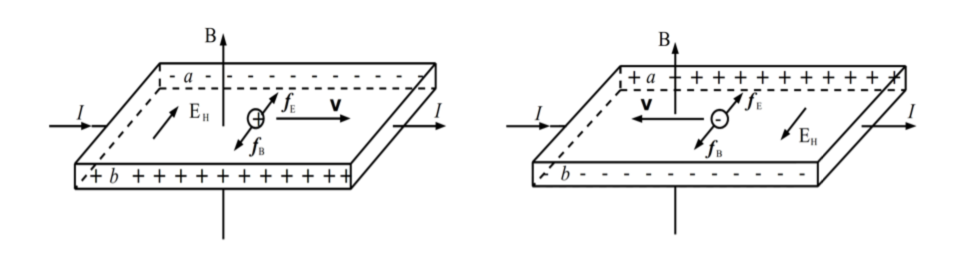
\includegraphics[width=0.9\textwidth]{Fig1} 
    \caption{The principle of the Hall effect.\cite{labmanual}} 
\end{figure}

If we view the Hall effect microscopically, we will find that it is actually caused by the Lorentz force $F_B$, which leads the deflection of moving charges. As a result, the accumulation of the charges on one side of the sheet increases the transverse electric field's magnitude (denoted by the Hall field $E_H$). However, because of the effect of the field, an electron force force $F_E$ in the charges will act upon the opposite direction of $F_B$. Eventually, a balance will be reached such that the net force of $F_E$ and $F_B$ is zero. At that time, $U_H$ stabilizes. Hence, we are able to determine the type of charge carriers in semiconductors by the analysis of the sign of $U_H$.

Further more, we find that when the external magnetic field is not strong to a certain extent, we have the following relationship between the magnitude of the magnetic field $B$, current $I$ and the thickness of the sheet $d$ shown in Eq.(1):
\begin{equation}
U_{\mathrm{H}}=R_{\mathrm{H}} \frac{I B}{d}=K I B
\end{equation}
where we call $R_H$ as the Hall coefficient and $K_H$ as the sensitivity of the Hall element. Here $K = R_H/d = K_H/I$. From the equation, we find that the Hall voltage is proportional to $I$ and $B$, and is inverse proportional to $d$. 
\subsection{\textsc{Integrated Hall Probe}}
If we fix the sensitivity $K_H$ and the current $I$, the magnitude of the magnetic field $B$ can be calculated accordingly by measuring the Hall voltage $U_H$. However, for the reason that the Hall voltage is small, we need to amplify the Hall voltage before measuring it.

The integrated Hall probe is a device which includes the Hall probe and the electric circuits as a single device. The probe we use in this lab is SS495A, which consists of a Hall sensor, an amplifier and a voltage compensator used to make the voltage stable and compensate for the differences (Figure 2).

As shown in Fig.2, the working voltage $U_S$ = 5V with output voltage $U_0$ approximately equals to 2.5V when the magnetic field is zero (Figure 2). The relation between the output voltage $U$ and the magnitude of the magnetic field $B$ can be written as follows:
\begin{equation}
B = \frac{U - U_0}{K_H}
\end{equation}

\begin{figure}[htb] 
    \centering
    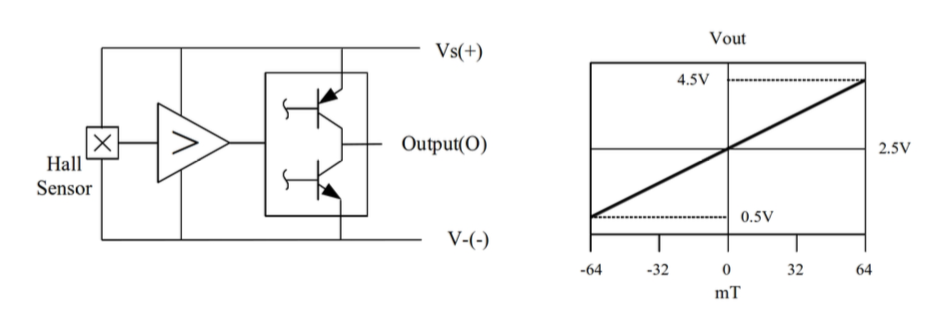
\includegraphics[width=0.9\textwidth]{Fig2} 
    \caption{The integrated Hall probe SS495A (left) and the relationship between $U$ and $B$ (right).\cite{labmanual}} 
\end{figure}

\subsection{\textsc{Magnetic Field Distribution Inside a Solenoid}}
The magnetic field distribution on the axis of a single layer solenoid is given by the following formula:
\begin{equation}
B(x)=\mu_{0} \frac{N}{L} I_{\mathrm{M}}\left\{\frac{L+2 x}{2\left[D^{2}+(L+2 x)^{2}\right]^{\frac{1}{2}}}+\frac{L-2 x}{2\left[D^{2}+(L-2 x)^{2}\right]^{\frac{1}{2}}}\right\}=C(x) I_{\mathrm{M}}
\end{equation}
where $I_M$ is the current through the solenoid wire, $L$ is the length, $N$ is the number of turns of the solenoid, and $D$ is the diameter of the solenoid. Moreover, $\mu_0 = 4\pi \times 10^{-7} H/m $ in the equation is the magnetic permeability of vacuum.

The solenoid we use in the lab has ten layers. According to Eq.(3), we obtained theoretical value of the magnetic field inside the solenoid when $I_M = 0.1A$. The details are shown in Table 1.

\begin{table}[H]
\begin{center}
\begin{tabular}{|c|c||c|c|}
\hline
x {[}cm{]} & B{[}mT{]} & x {[}cm{]} & B {[}mT{]} \\ \hline
$\pm$ 0.0 & 1.4366 & $\pm$ 8.0 & 1.4057 \\ \hline
$\pm$ 1.0 & 1.4364 & $\pm$ 9.0 & 1.3856 \\ \hline
$\pm$ 2.0 & 1.4356 & $\pm$ 10.0 & 1.3478 \\ \hline
$\pm$ 3.0 & 1.4343 & $\pm$ 11.0 & 1.2685 \\ \hline
$\pm$ 4.0 & 1.4323 & $\pm$ 11.5 & 1.1963 \\ \hline
$\pm$ 5.0 & 1,4292 & $\pm$ 12.0 & 1.0863 \\ \hline
$\pm$ 6.0 & 1.4245 & $\pm$ 12.5 & 0.9261 \\ \hline
$\pm$ 7.0 & 1.4173 & $\pm$ 13.0 & 0.7233 \\ \hline
\end{tabular}
\caption{Theoretical value of the magnetic field inside the solenoid.\cite{labmanual}}
\end{center}
\end{table}

\subsection{\textsc{Study of the Geomagnetic Field with a Hall Probe}}
\begin{figure}[htb] 
    \centering
    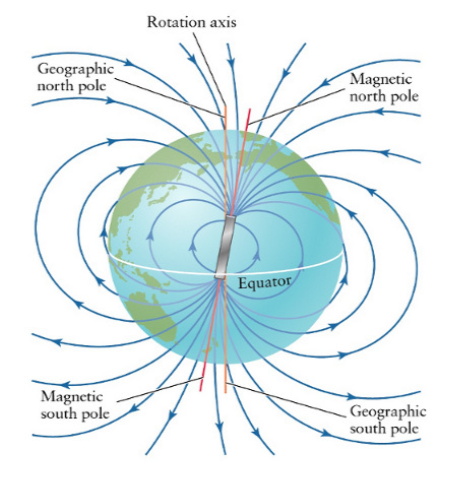
\includegraphics[width=0.45\textwidth]{Fig3} 
    \caption{Magnetic field of the Earth.\cite{labmanual}} 
\end{figure}

\begin{figure}[htb] 
    \centering
    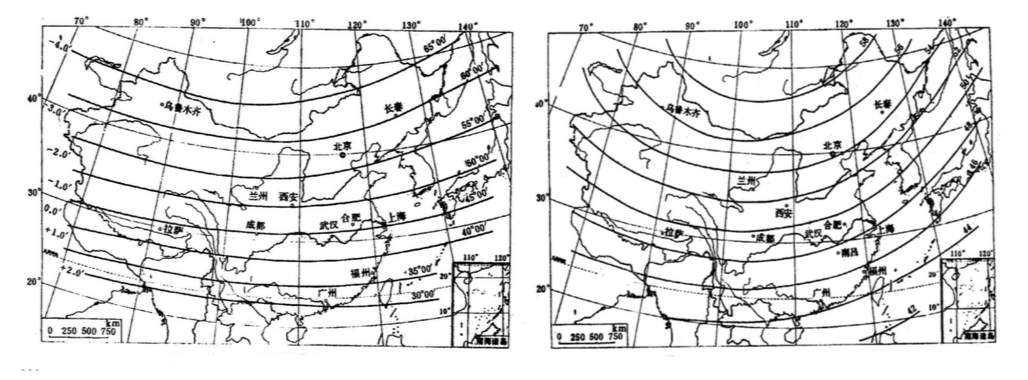
\includegraphics[width=0.8\textwidth]{Fig4} 
    \caption{Geomagnetic inclination (1970) (left). The magnitude of geomagnetic field (right).\cite{labmanual}} 
\end{figure}
As shown in Fig.3, we can see that the geomagnetic field as an analogue to that of a bar magnet tilted about 11.5$^{\circ}$ from the spin axis of the Earth. Consequently, the "bar magnet" forms the geomagnetic field.

In Fig.4, we see the geomagnetic field distribution of China in 1970. The magnetic inclination is 44.5$^{\circ}$ with the corresponding magnetic field in Shanghai 48000nT.
%----------------------------------------------------------------------------------------
%	SECTION 3
%----------------------------------------------------------------------------------------
\section{\textsc{Apparatus and Experimental Setup}}
We set up the experiment as shown in Fig.5. Fig.6 shows the integrated Hall probe SS495A we use. In all, the apparatuses we use in this lab are listed below:
\begin{itemize}
\item An integrated Hall probe SS495A with $K_H = 31.25 \pm 1.25 V/T$ at the working voltage 5 V.
\item A solenoid.
\item A power supply.
\item A voltmeter.
\item A DC voltage divider.
\item A set of connecting wires.
\end{itemize}
\begin{figure}[H] 
    \centering
    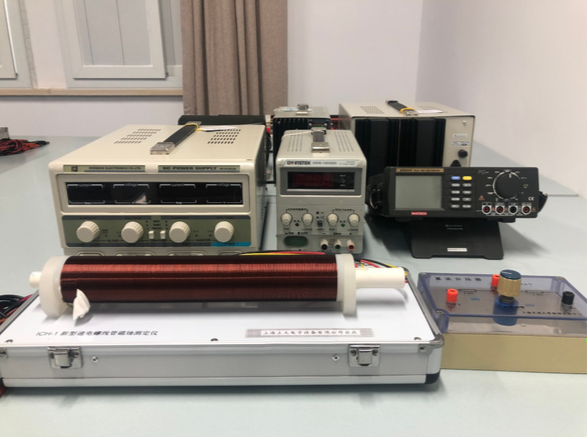
\includegraphics[width=0.55\textwidth]{Fig5} 
    \caption{Measurement setup.\cite{labmanual}} 
\end{figure}

\begin{figure}[H] 
    \centering
    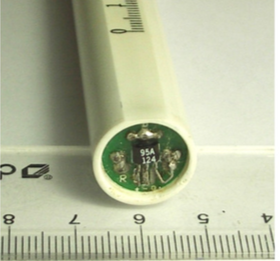
\includegraphics[width=0.3\textwidth]{Fig6} 
    \caption{Integrated Hall probe SS495A.\cite{labmanual}} 
\end{figure}

Then, the uncertainties for the quantities we measured in this lab are listed in Table 2:

\begin{table}[H]
\begin{center}
\begin{tabular}{|c|c|}
\hline
Quantity & Uncertainty \\ \hline
$U_S$ (voltage source) & 0.5\% {[}V{]} \\ \hline
$U_0$ \& $U$ (voltimeter) & 0.05\% + $6\times 10^{-3}$ or $6\times 10^{-4}$ {[}V{]} \\ \hline
$I_M$ (current source) & 2\% {[}mA{]} \\ \hline
x (distance) & 0.05 {[}cm{]} \\ \hline
\end{tabular}
\caption{Uncertainties of quantities measured in this lab.}
\end{center}
\end{table}
Note that for $U_0$ \& $U$, the uncertainty depends, and we choose the correct uncertainty accordingly.

%----------------------------------------------------------------------------------------
%	SECTION 4
%----------------------------------------------------------------------------------------
\section{\textsc{Procedures \cite{labmanual}}}
\subsection{\textsc{Relation Between Sensitivity $K_H$ and Working Voltage $U_S$}}
\begin{itemize}
\item[1.] First, we place the integrated Hall probe at the center of the solenoid.
\item[2.] Second, we set the working voltage at 5 V and measure the output voltage $U_0$ ($I_M$ = 0) and U ($I_M$ = 250 mA).
\item[3.] Third, we take the theoretical value of B(x = 0) from Table 1 and calculate the sensitivity of the probe $K_H$ by using Eq. (2).
\item[4.] Eventually, we measure $K_H$ for different values of $U_S$ (from 2.8 V to 10 V). Calculate $K_H$/$U_S$ and plot the curve $K_H$/$U_S$ vs. $U_S$.
\end{itemize}

\subsection{\textsc{Relation Between Output Voltage U and Magnetic Field B}}
\begin{itemize}
\item[1.] First, we connect the 2.4 - 2.6 V output terminal of the DC voltage divider and the negative port of the voltmeter with B=0 and $U_S$=5 V. Then adjust the voltage until $U_0$ = 0.
\item[2.] Second, we place the integrated Hall probe at the center of the solenoid and measure the output voltage U for different values of $I_M$ ranging from 0 to 500 mA, with intervals of 50 mA.
\item[3.] Third, we explain the relation between B(x = 0) and the Hall voltage $U_H$. Notice that the output voltage has been amplified and the theoretical value of B(x = 0) can be found from introduction part.
\item[4.] Finally, we plot the curve U vs. B and find the sensitivity $K_H$ through linear fit. Compare the value with (1) the theoretical one (2) the value in first part.
\end{itemize}

\subsection{\textsc{Magnetic Field Distribution Inside the Solenoid}}
\begin{itemize}
\item[1.] First, we measure the magnetic field distribution along the axis of the solenoid under the condition that $I_M$ = 250mA. Then we record the output voltage U and position x and find out B = B(x). by using $K_H$ we obtain in first part.
\item[2.] Then, we plot the theoretical and experimental curve to show the magnetic field distribution inside the solenoid. Note that for experimental curve we use dot points and for the theoretical one we use solid line.
\end{itemize}

\subsection{\textsc{Measurement of the Geomagnetic Field}}
\begin{itemize}
\item[1.] We use an integrated Hall probe to measure both the magnitude and the direction of the geomagnetic field.
\end{itemize}
%----------------------------------------------------------------------------------------
%	SECTION 5
%----------------------------------------------------------------------------------------
\section{\textsc{Results}}
\subsection{\textsc{Relation Between Sensitivity $K_H$ and Working Voltage $U_S$}}
In this part, we find out the relation between sensitivity $K_H$ and working voltage $U_S$. The data is recorded in Table 3.
\begin{table}[H]
\begin{center}
\begin{tabular}{|c|c|c|}
\hline
$U_S$ {[}V{]} $\pm$ 0.5\% {[}V{]} & \begin{tabular}[c]{@{}c@{}}$U_0$ ($I_M$ = 0) {[}V{]} $\pm$ \\ 0.05\% + $6\times 10^{-3}$/$6\times 10^{-4}$ {[}V{]}\end{tabular} & \begin{tabular}[c]{@{}c@{}}$U$ ($I_M$ = 250 mA) {[}V{]} $\pm$ \\ 0.05\% + $6\times 10^{-3}$/$6\times 10^{-4}$ {[}V{]}\end{tabular} \\ \hline
5.00 & 2.482 & 2.602 \\ \hline
\end{tabular}
\caption{Data for $U_0$ and U with $U_S$ = 5 V.}
\end{center}
\end{table}

To proceed, we need to first find out the value of $K_H$ based on Eq.(2) and Table 1. From Table 1, we know that when $I_{M,t}$ = 0.1 A, the magnetic field in the middle of the solenoid is B = 1.4366 mT. 
\par However, in this section, when measuring, the real current we choose is $I_{M,r}$ = 250 mA. Hence, we ought to find out the theoretical value of B at $I_M$ = 250 mA = 0.25 A. Accordingly to Eq.(2), we have:
\begin{center}
$\displaystyle B_{M} = B \times \frac{I_{M,r}}{I_{M,t}} = 1.4366 \times \frac{0.25}{0.1} = 3.5915 [mT] $
\end{center}
Note that this is the calculation based on the theoretical values. Hence no uncertainty is generated here.
\par Then, based on our results, we are able to find out the sensitivity of the probe $K_H$ as follows (Detailed calculations of uncertainties are shown in A.1):
\begin{center}
$\displaystyle K_H = \frac{U-U_0}{B_M} = \frac{2.602 - 2.482}{3.5915} = 0.033 \pm 0.003 [kV/T]$
\end{center} 
with a relative uncertainty $r_{K_H}$ = 9\%.

\newpage
\par Then, we are going to find out $K_H$ for different values of $U_S$ varying from 2.8 V to 10 V through Eq.(2) and then find out $\frac{K_H}{U_S}$.
\par Take $U_S$ = 2.80 V as an example, and we will obtain $\frac{K_H}{U_S}$ at this voltage is (Detailed calculations of uncertainties are shown in A.1):
\begin{center}
$\displaystyle \frac{K_H}{U_S} = \frac{U-U_0}{B_M U_S} = \frac{1.4694 - 1.4019}{3.5915 \times 2.80} = 0.00671 \pm 0.00019 [mT^{-1}] $ 
\end{center}
with a relative uncertainty $r_{K_H/U_S}$ = 3\%.
\par Now, we do the same calculations for all the 18 pairs of data we collected, and we will obtain Table 4:
\begin{table}[H]
\begin{center}
\begin{tabular}{|c|c|c|c|c|c|c|}
\hline
 & \begin{tabular}[c]{@{}c@{}}$U_S$ {[}V{]} $\pm$\\ 0.5\% {[}V{]}\end{tabular} & $u_{U_S}$ & \begin{tabular}[c]{@{}c@{}}$U_0$ {[}V{]} $\pm$ 0.05\% +\\ $6\times 10^{-4}/6\times 10^{-3}$ {[}V{]}\end{tabular} & \begin{tabular}[c]{@{}c@{}}$U$ {[}V{]} $\pm$ 0.05\% +\\ $6\times 10^{-4}/6\times 10^{-3}$ {[}V{]}\end{tabular} & $\frac{K_H}{U_S}$ & $u_{\frac{K_H}{U_S}}$ \\ \hline
1 & 2.800 & 0.014 & 1.4019 & 1.4694 & 0.00671 & 0.00019 \\ \hline
2 & 3.200 & 0.016 & 1.5977 & 1.6767 & 0.00687 & 0.00017 \\ \hline
3 & 3.600 & 0.018 & 1.7970 & 1.8848 & 0.00679 & 0.00017 \\ \hline
4 & 4.00 & 0.02 & 1.9922 & 2.0893 & 0.00676 & 0.00016 \\ \hline
5 & 4.40 & 0.02 & 2.186 & 2.292 & 0.0067 & 0.0006 \\ \hline
6 & 4.80 & 0.02 & 2.382 & 2.495 & 0.0066 & 0.0006 \\ \hline
7 & 5.20 & 0.03 & 2.577 & 2.700 & 0.0066 & 0.0006 \\ \hline
8 & 5.60 & 0.03 & 2.772 & 2.905 & 0.0066 & 0.0005 \\ \hline
9 & 6.00 & 0.03 & 2.966 & 3.107 & 0.0065 & 0.0005 \\ \hline
10 & 6.40 & 0.03 & 3.160 & 3.306 & 0.0064 & 0.0005 \\ \hline
11 & 6.80 & 0.03 & 3.351 & 3.504 & 0.0063 & 0.0004 \\ \hline
12 & 7.20 & 0.04 & 3.541 & 3.700 & 0.0061 & 0.0004 \\ \hline
13 & 7.60 & 0.04 & 3.735 & 3.901 & 0.0061 & 0.0004 \\ \hline
14 & 8.00 & 0.04 & 3.929 & 4.097 & 0.0058 & 0.0004 \\ \hline
15 & 8.40 & 0.04 &4.120 & 4.292 & 0.0057 & 0.0004 \\ \hline
16 & 8.80 & 0.04 & 4.309 & 4.480 & 0.0054 & 0.0004 \\ \hline
17 & 9.40 & 0.04 & 4.593 & 4.767 & 0.0052 & 0.0003 \\ \hline
18 & 10.00 & 0.05 & 4.880 & 5.061 & 0.0050 & 0.0003 \\ \hline
\end{tabular}
\caption{Data for $U_0$ and U with different $U_S$.}
\end{center}
\end{table}

Now, we are able to use \textit{Origin} to plot the curve $\frac{K_H}{U_S}$ vs. $U_S$ based on the data in Table 4. The result is shown in Fig.7. From the curve, we can observe that with the \textbf{increase} of $U_S$, $\frac{K_H}{U_S}$ has a general trend to \textbf{decrease}.

\newpage
\begin{figure}[H] 
    \centering
    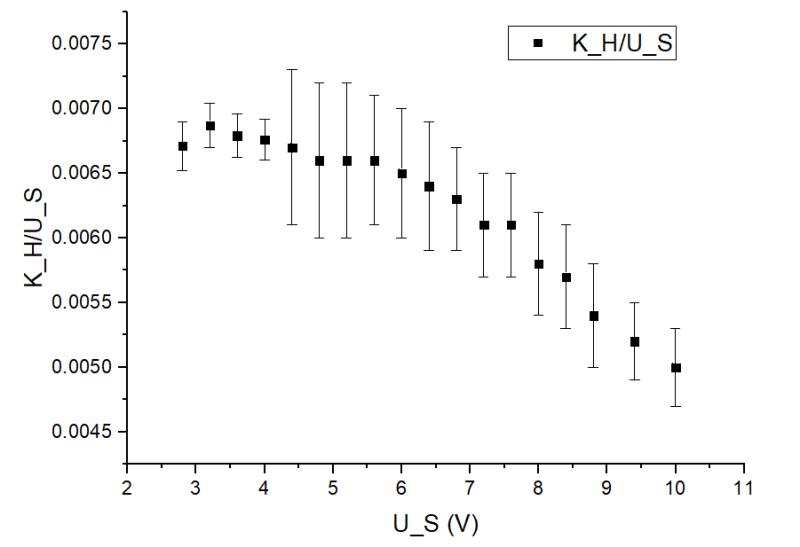
\includegraphics[width=0.67\textwidth]{p1} 
    \caption{$\frac{K_H}{U_S}$ vs. $U_S$.} 
\end{figure}




\subsection{\textsc{Relation Between Output Voltage U and Magnetic Field B}}
According to Eq.(3), we have the following formula:
\begin{center}
$\displaystyle C(x) = \frac{B(x)}{I_M} $
\end{center}
Based on the data in Table 1, we are able to obtain the value of C(x) when x = 0 as follows:
\begin{center}
$\displaystyle C(x) = \frac{1.4366}{0.1} = 14.366 [mT/A] $
\end{center}
Now, we are able to find out B through C(x) and $I_M$, where $I_M$ is the value we measured in the lab. Then, we are able to obtain the data in Table 5.
\begin{table}[H]
\begin{center}
\begin{tabular}{|c|c|c|c|c|c|}
\hline
 & $I_M$ {[}mA{]} $\pm$ 2\% {[}mA{]} & U {[}V{]} $\pm$ 0.05\% + $6\times10^{-4}$ {[}V{]} & $u_U$ & B {[}mT{]} & $u_B$ {[}mT{]} \\ \hline
1 & 0 & 0.0000 & 0.0006 & 0 & 0 \\ \hline
2 & 50 & 0.0256 & 0.0006 & 0.718 & 0.014 \\ \hline
3 & 100 & 0.0510 & 0.0006 & 1.44 & 0.03 \\ \hline
4 & 150 & 0.0731 & 0.0006 & 2.15 & 0.04 \\ \hline
5 & 200 & 0.0974 & 0.0006 & 2.87 & 0.06 \\ \hline
6 & 250 & 0.1205 & 0.0007 & 3.59 & 0.07 \\ \hline
7 & 300 & 0.1419 & 0.0007 & 4.31 & 0.09 \\ \hline
8 & 350 & 0.1664 & 0.0007 & 5.03 & 0.10 \\ \hline
9 & 400 & 0.1856 & 0.0007 & 5.75 & 0.12 \\ \hline
10 & 450 & 0.2102 & 0.0007 & 6.46 & 0.13 \\ \hline
11 & 500 & 0.2324 & 0.0007 & 7.18 & 0.14 \\ \hline
\end{tabular}
\caption{Measurement data for the $I_M$ vs. $U$ relation.}
\end{center}
\end{table}

\newpage
As sample calculation, we choose the data when $I_M$ = 50 mA, and we have (Detailed calculations of uncertainties are shown in A.2):
\begin{center}
$\displaystyle B = C(x) \times I_M = 14.366 \times 50 \times 10^{-3} = 0.718 \pm 0.014 [mT] $
\end{center}
with a relative uncertainty 2\%.
\par Now, we are able to use \textit{Origin} to plot a linear fit for $U$ vs. $B$. The result is shown in Fig.8.
\begin{figure}[H] 
    \centering
    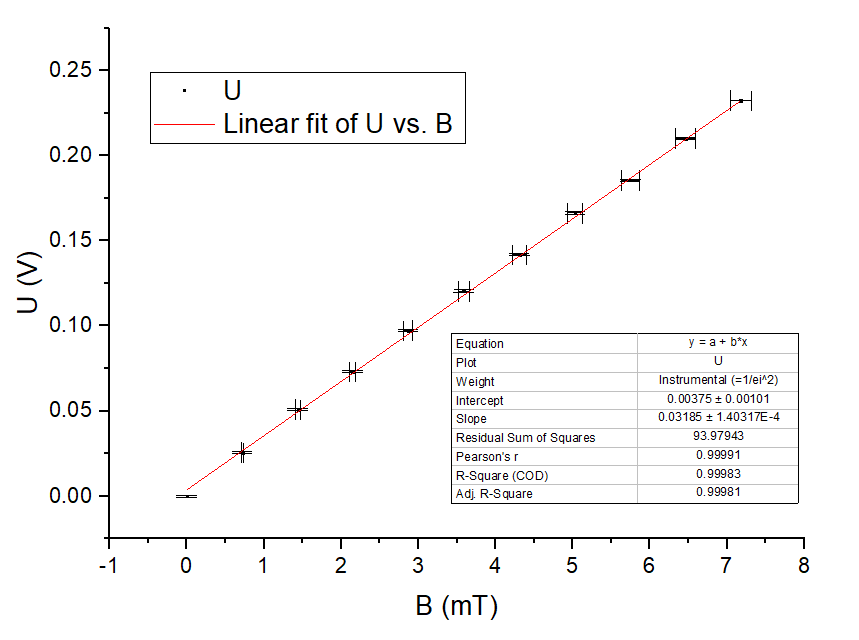
\includegraphics[width=0.75\textwidth]{p2} 
    \caption{$\frac{K_H}{U_S}$ vs. $U_S$.} 
\end{figure}
Since $U$ is the output signal of $U_H$, we can find out the relationship between $B$ and the Hall voltage $U_H$ through the figure. Since the Pearson's R is 0.99991, which is very close to 1, we can conclude that they do have a linear relationship.
\par Also, from the linear fit, we can obtain $K_H$ as:
\begin{center}
$ K_H = 0.0319 \pm 0.0003 [kV/T]$
\end{center}
with a relative uncertainty $r_{K_H} = 1.0\%$.
\par In the first part, the $K_H$ we obtain is $K_{H,1} = 0.033 \pm 0.003 [kV/T] $. We can find out their relative error is 3\%, which is acceptable, indicating that the two answers we obtain are very close to each other.



\subsection{\textsc{Magnetic Field Distribution Inside the Solenoid}}
In order to find out B(x), we can use the following formula:
\begin{center}
$ \displaystyle B = \frac{U}{K_H} $
\end{center}
where $K_H$ is what we have find out before.
\par Then, we collected 52 pairs of data, which is recorded in Table 6. For the calculation of B, we take the case when x = 0 [cm] as a sample calculation (Detailed calculations of uncertainties are shown in A.3):
\begin{center}
$ \displaystyle B = \frac{U}{K_H} = \frac{0.0097}{0.0319 \times 10^3} = 0.00030 \pm 0.00002 [mT] $
\end{center}

\begin{table}[H]
\begin{center}
\resizebox{\textwidth}{75mm}{
\begin{tabular}{|c|c|c|c|c||c|c|c|c|c|}
\hline
 & \begin{tabular}[c]{@{}c@{}}x {[}cm{]} $\pm$\\ 0.05 {[}cm{]}\end{tabular} & \begin{tabular}[c]{@{}c@{}}U {[}V{]} $\pm$ 0.05\%\\ + $6\times 10^{-4}$ {[}V{]}\end{tabular} & B {[}mT{]} & $u_B$ &  & \begin{tabular}[c]{@{}c@{}}x {[}cm{]} $\pm$\\ 0.05 {[}cm{]}\end{tabular} & \begin{tabular}[c]{@{}c@{}}U {[}V{]} $\pm$ 0.05\%\\ + $6\times 10^{-4}$ {[}V{]}\end{tabular} & B {[}mT{]} & $u_B$ \\ \hline
1 & 0.0 & 0.0097 & 0.304 & 0.019 & 27 & 18.0 & 0.1201 & 3.76 & 0.03 \\ \hline
2 & 0.2 & 0.0119 & 0.373 & 0.019 & 28 & 19.0 & 0.1200 & 3.76 & 0.03 \\ \hline
3 & 0.4 & 0.0136 & 0.426 & 0.019 & 29 & 20.0 & 0.1200 & 3.76 & 0.03 \\ \hline
4 & 0.6 & 0.0150 & 0.470 & 0.019 & 30 & 21.0 & 0.1200 & 3.76 & 0.03 \\ \hline
5 & 0.8 & 0.0173 & 0.542 & 0.019 & 31 & 22.0 & 0.1195 & 3.75 & 0.03 \\ \hline
6 & 1.0 & 0.0194 & 0.608 & 0.019 & 32 & 23.0 & 0.1187 & 3.72 & 0.03 \\ \hline
7 & 1.2 & 0.0227 & 0.712 & 0.019 & 33 & 24.0 & 0.1170 & 3.67 & 0.03 \\ \hline
8 & 1.4 & 0.0248 & 0.777 & 0.019 & 34 & 25.0 & 0.1158 & 3.63 & 0.03 \\ \hline
9 & 1.6 & 0.0286 & 0.897 & 0.019 & 35 & 26.0 & 0.1123 & 3.52 & 0.03 \\ \hline
10 & 1.8 & 0.0335 & 1.050 & 0.019 & 36 & 26.2 & 0.1112 & 3.49 & 0.03 \\ \hline
11 & 2.0 & 0.0383 & 1.201 & 0.019 & 37 & 26.4 & 0.1097 & 3.44 & 0.03 \\ \hline
12 & 3.0 & 0.0707 & 2.22 & 0.02 & 38 & 26.6 & 0.1064 & 3.34 & 0.02 \\ \hline
13 & 4.0 & 0.0965 & 3.03 & 0.02 & 39 & 26.8 & 0.1064 & 3.34 & 0.02 \\ \hline
14 & 5.0 & 0.1098 & 3.44 & 0.03 & 40 & 27.2 & 0.1013 & 3.18 & 0.02 \\ \hline
15 & 6.0 & 0.1149 & 3.60 & 0.03 & 41 & 27.6 & 0.0945 & 2.96 & 0.02 \\ \hline
16 & 7.0 & 0.1176 & 3.69 & 0.03 & 42 & 28.0 & 0.0854 & 2.68 & 0.02 \\ \hline
17 & 8.0 & 0.1181 & 3.70 & 0.03 & 43 & 28.2 & 0.0781 & 2.45 & 0.02 \\ \hline
18 & 9.0 & 0.1185 & 3.71 & 0.03 & 44 & 28.4 & 0.0736 & 2.31 & 0.02 \\ \hline
19 & 10.0 & 0.1202 & 3.77 & 0.03 & 45 & 28.6 & 0.0656 & 2.06 & 0.02 \\ \hline
20 & 11.0 & 0.1205 & 3.78 & 0.03 & 46 & 28.8 & 0.0591 & 1.85 & 0.02 \\ \hline
21 & 12.0 & 0.1204 & 3.77 & 0.03 & 47 & 29.0 & 0.0515 & 1.61 & 0.02 \\ \hline
22 & 13.0 & 0.1206 & 3.78 & 0.03 & 48 & 29.2 & 0.0463 & 1.45 & 0.02 \\ \hline
23 & 14.0 & 0.1203 & 3.77 & 0.03 & 49 & 29.4 & 0.0384 & 1.204 & 0.019 \\ \hline
24 & 15.0 & 0.1205 &  3.78 & 0.03 & 50 & 29.6 & 0.0345 & 1.082 & 0.019 \\ \hline
25 & 16.0 & 0.1205 &  3.78 & 0.03 & 51 & 29.8 & 0.0298 & 0.934 & 0.019 \\ \hline
26 & 17.0 & 0.1204 &  3.77 & 0.03 & 51 & 30.0 & 0.0252 & 0.790 & 0.019 \\ \hline
\end{tabular}
}
\caption{Measurement data for the $I_M$ vs. $U$ relation.}
\end{center}
\end{table}

Then, we derive the theoretical value based on Table 1. As what we have done in the first part, since B is in proportional to $I_M$, we are able to find out the value of $B$ when $I_M$ = 0.25 A. The result is shown in Table 7.

\par Hence, with the data in Table 6 and Table 7, we can use \textit{Origin} to plot the theoretical and experimental value of B vs. x. The curve is shown in Fig.9.

\newpage

\begin{table}[H]
\begin{center}
\begin{tabular}{|c|c|c||c|c|c|}
\hline
x {[}cm{]} & B{[}mT{]} & $B_M${[}mT{]} & x {[}cm{]} & B {[}mT{]} & $B_M${[}mT{]} \\ \hline
$\pm$ 0.0 & 1.4366 & 3.5915 & $\pm$ 8.0 & 1.4057 & 3.5143 \\ \hline
$\pm$ 1.0 & 1.4364 & 3.5908 & $\pm$ 9.0 & 1.3856 & 3.4640\\ \hline
$\pm$ 2.0 & 1.4356 & 3.5890 & $\pm$ 10.0 & 1.3478 & 3.3695\\ \hline
$\pm$ 3.0 & 1.4343 & 3.5858 & $\pm$ 11.0 & 1.2685 & 3.1713\\ \hline
$\pm$ 4.0 & 1.4323 & 3.5808 & $\pm$ 11.5 & 1.1963 & 2.9908\\ \hline
$\pm$ 5.0 & 1,4292 & 3.5730 & $\pm$ 12.0 & 1.0863 & 2.7158\\ \hline
$\pm$ 6.0 & 1.4245 & 3.5613 & $\pm$ 12.5 & 0.9261 & 2.3153\\ \hline
$\pm$ 7.0 & 1.4173 & 3.5433 & $\pm$ 13.0 & 0.7233 & 1.8083\\ \hline
\end{tabular}
\caption{Theoretical value of the magnetic field when $I_M$ = 250 mA.}
\end{center}
\end{table}


\begin{figure}[H] 
    \centering
    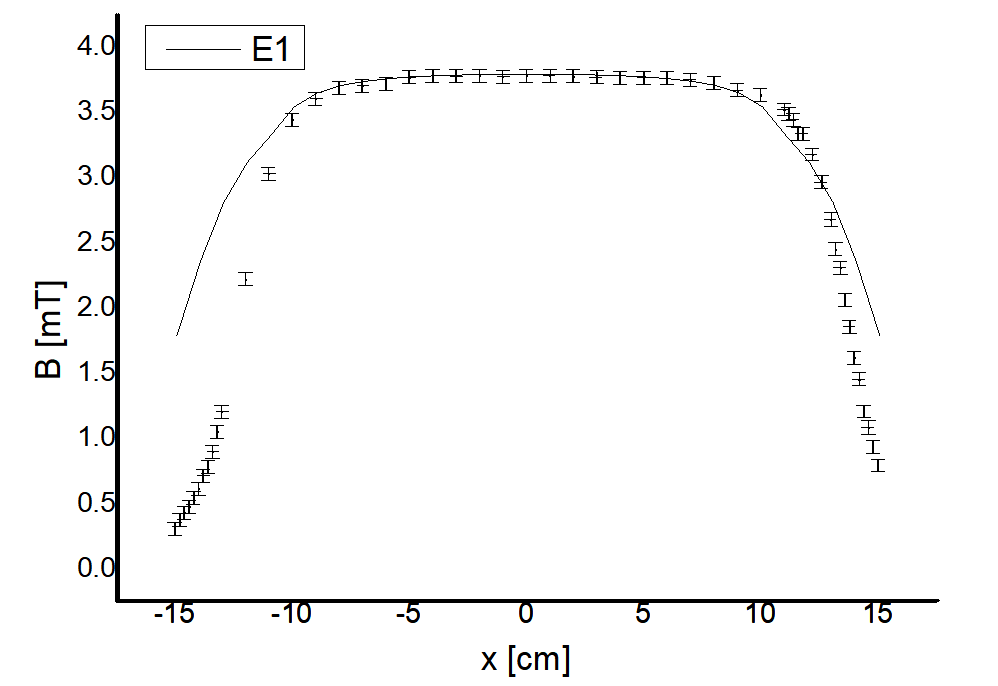
\includegraphics[width=0.8\textwidth]{p3} 
    \caption{Magnetic field distribution inside the solenoid.} 
\end{figure}

%----------------------------------------------------------------------------------------
%	SECTION 6
%----------------------------------------------------------------------------------------
\newpage
\section{\textsc{Conclusion and Discussion}}
\subsection{\textsc{Discussion}}
In this lab, generally speaking we have done a successful job. However, there are still some sources of error. The sources of error and their corresponding solutions are listed below:
\begin{itemize}
\item[1.] In the part "Relation Between Sensitivity $K_H$ and Working Voltage $U_S$":
	\begin{itemize}
	\item When measuring, we measure the voltage only once, which may lead to a relatively large error while applying Eq.(2).
	
			[Solution]: We can measure the voltage for multiple times and calculate the answer. Then by taking the average we can reduce the error.
			
	\item In Fig.7, though our result is satisfactory overall, it still exist some error. It may come from the time when we are adjusting the apparatuses.
		
			[Solution]: Under the process of the experiment, we should adjust the apparatuses as less as possible to reduce the error.
	\end{itemize}
	
\item[2.] In the part "Relation Between Output Voltage U and Magnetic Field B":
	\begin{itemize}
	\item In this part, we have some little errors. This is because when calculating the magnetic field B, we should use C(x). Hence if C(x) has error, our result will be affected accordingly.
	
			[Solution]: We can record more groups of data and find out C(x) by taking the average. In this way the error can be reduced.
	\end{itemize}
	
\item[3.] In the part "Magnetic Field Distribution Inside the Solenoid":
\par 	In this part, plot the magnetic field distribution inside the solenoid. The general shape of our result is similar to that of the theoretical one. However, some error still exists. It may be caused by:
	\begin{itemize}
	\item When the Hall probe are in the two sides, the value of magnetic field changes rapidly, which may cause the error.
	
	[Solution]: We can record more groups of data when the Hall probe is near the two sides.
	\item The theoretical value we use in this lab is measured when $I_M$ = 0.1 A. However, in this lab our $I_M$ = 0.25 A. Although we have changed the scale, some errors may still occur.
	
	[Solution]: We can either find a theoretical with $I_M$ = 0.25 A, or in the experiment we simply choose $I_M$ = 0.1 A.
	\end{itemize}

\item[4.] When measuring the values near the two sides, the Hall probe will have a small inclination. In other words, the Hall probe is not horizontal to the ground. This may leads to error. The case is shown in FIg.10.

	[Solution]: We can improve the stability if the apparatus. In other words, we can build the probe stronger.

\begin{figure}[H] 
    \centering
    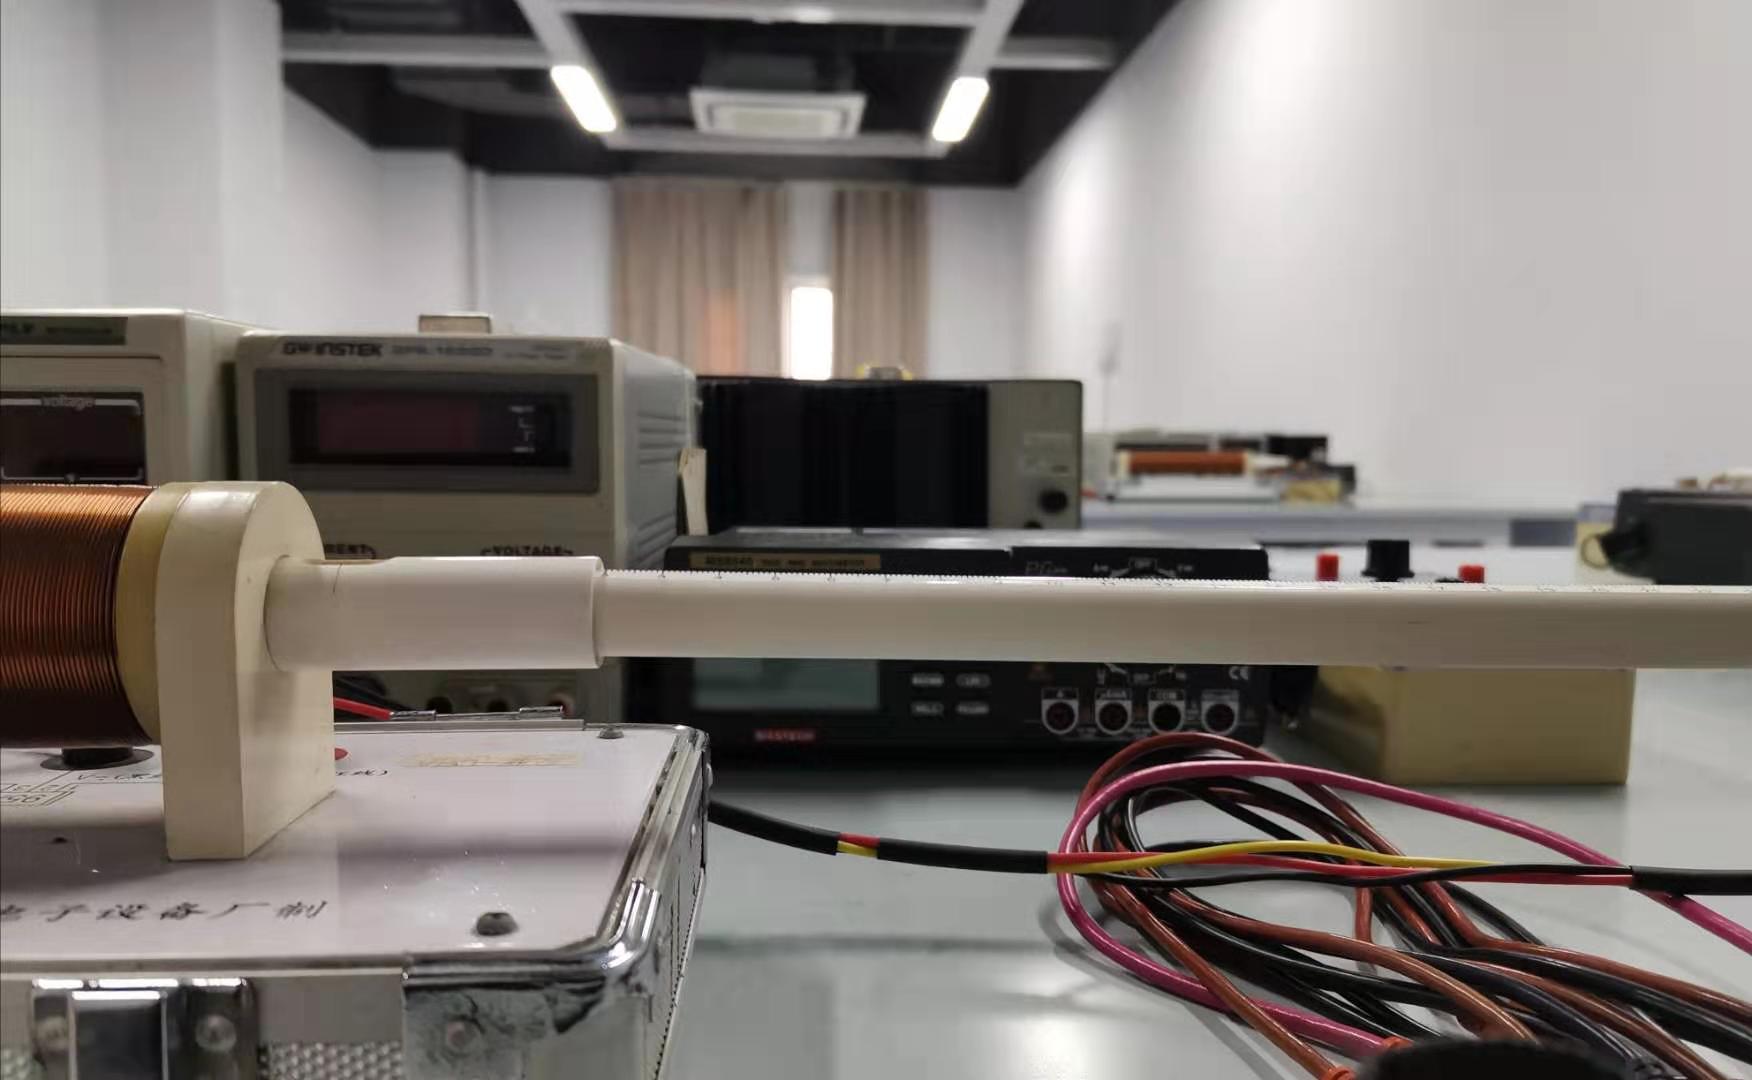
\includegraphics[width=0.7\textwidth]{p4} 
    \caption{The Hall probe is not perfectly horizontal, and is inclined for a small angle.} 
\end{figure}

\item[5.] When connecting the circuit, the wire, and even the solenoid has a small resistance. However, in this lab we just ignore them.

	[Solution]: We can take into consideration the resistance of the wires.
	
\item[6.] When we read the values on the screen, the readings is not stable and is always oscillating. The phenomenon is particularly obvious when the values are small.

	[Solution]: We can wait for a longer time until the reading is stable.
\end{itemize}

\subsection{\textsc{Conclusion}}
In this lab, I have really learned a lot. We successfully fulfil the objectives, and find out the following phenomenon:
\begin{itemize}
\item With the increase of $U_S$, $\displaystyle \frac{K_H}{U_S}$ has a general trend to decrease.
\item The Hall voltage is proportional to the magnetic field.
\item Inside the solenoid, we find that the magnetic field is the largest in the middle and decrease when going to the sides. The decrease is rapid near the two sides.
\item The quantities of Hall probe and their relationships.
\end{itemize}
Also, I learned the following after the lab:
\begin{itemize}
\item The principle of the Hall effect.
\item The applications of how to use a Hall probe.
\item How to discover the magnetic field of a solenoid.
\end{itemize}
Furthermore, we can use a Hall probe to detect the magnetic field on the Earth.

%----------------------------------------------------------------------------------------
%	SECTION 7
%----------------------------------------------------------------------------------------

\begin{appendices} 
\section{\textsc{Measurement uncertainty analysis}} 
\subsection{\textsc{Relation Between Sensitivity $K_H$ and Working Voltage $U_S$}} 
Since $K_H$ is calculated through $ K_H = (U-U_0)/B_M $, the uncertainty $u_{K_H}$can be find out by using uncertainty propagation formula:
\begin{center}
$\displaystyle u_{K_H} = \sqrt{(\frac{\partial K_H}{\partial U})^2(u_U)^2 + (\frac{\partial K_H}{\partial U_0})^2(u_{U_0})^2} = \frac{\sqrt{u_U^2 + u_{U_0}^2}}{B_M}$ 
\end{center}
Hence, by plugging in the values, we obtain:
\begin{center}
$\displaystyle U_{K_H} = \frac{ \sqrt{(2.482 \times 0.05\% + 6\times 10^{-3})^2 + (2.602 \times 0.05\% + 6\times 10^{-3})^2} }{3.5915} = 0.003 [kV/T] $
\end{center}
\par Hence, $K_H$ can be written as:
\begin{center}
$ K_H = 0.033 \pm 0.003 [kV/T] $
\end{center}

\par Then, we need to calculate the uncertainty of $\frac{K_H}{U_S}$. Since $\frac{K_H}{U_S}$ is calculated through $\frac{K_H}{U_S} = \frac{U-U_0}{B_M U_S}$, the uncertainty $u_{K_H/U_S}$can be find out by using uncertainty propagation formula similarly. Take $U_S$ = 2.80 V as an example, and we will obtain:
\begin{center}
$\begin{aligned} 
u_{K_H/U_S} &=\sqrt{(\frac{\partial f}{\partial U})^2(u_U)^2 + (\frac{\partial f}{\partial U_0})^2(u_{U_0})^2 + (\frac{\partial f}{\partial U_S})^2(u_{U_S})^2} \\ 
				&=\sqrt{\left(\frac{1}{B_M U_{S}} u_{U}\right)^{2}+\left(\frac{1}{B_M U_{S}} u_{U_{0}}\right)^{2}+\left(\frac{U-U_{0}}{B_M U_{S}^{2}} \times u_{U_{S}}\right)^{2}} \\ 
				&=\sqrt{\left(\frac{1}{3.5915 \times 2.8} \times u_{U}\right)^{2}+\left(\frac{1}{3.5915 \times 2.8} \times u_{U_{0}}\right)^{2}+\left(\frac{1.4694-1.4019}{3.5915 \times 2.8^{2}} \times 2.8 \times 0.5 \%\right)^{2}} \\ 
				&=0.00019 [mT^{-1}] 
\end{aligned} $
\end{center}
Hence, the value of $K_H/U_S$ when $U_S$ = 2.80 V can be written as:
\begin{center}
$\displaystyle \frac{K_H}{U_S} = 0.00671 \pm 0.00019 [mT^{-1}] $ 
\end{center}

\subsection{\textsc{Relation Between Output Voltage U and Magnetic Field B}}
To calculate the uncertainty of $B$, we note that B is given by $B = C(x) \times I_M$, where C(x) is a constant and we do not need to take into consideration its uncertainty. Hence, the uncertainty of $B$ is simply the type-B uncertainty, which is shown as follows:
\begin{center}
$u_B = C(x) \times u_B$
\end{center}
Take the case when $I_M = 50 mA $ as a sample calculation, we will obtain:
\begin{center}
$u_B = 14.366 \times 2\% \times 0.05 = 0.014 [mT]$
\end{center}
And the other values can be calculated in exactly the same way.
\par To find out the uncertainty of the slope, we can calculate through the following formula:
\begin{center}
$ u = t_{0.95} \times Std = 2.26 \times 1.40317 \times 10^{-4} = 0.0003 [kV/T] $ 
\end{center}

\subsection{\textsc{Magnetic Field Distribution Inside the Solenoid}}
In this part, we calculate B through the following formula: $B = \frac{U}{K_H}$. Based on uncertainty propagation, we can find out the uncertainty of B as follows:
\begin{center}
$
\begin{aligned}
u_B &= \sqrt{(\frac{\partial B}{\partial U})^2(u_U)^2 + (\frac{\partial B}{\partial K_H})^2(u_{K_H})^2}\\
		&= \sqrt{\frac{1}{K_H^2}(u_U)^2 + \frac{U^2}{K_H^4}(u_{K_H})^2}
\end{aligned}
 $
\end{center}
Take the case when x = 0 [cm] as a sample calculation, and we will have:
\begin{center}
$\displaystyle  u_B = \sqrt{\frac{1}{31.9^2}(0.0097\times 0.05\% + 6\times 10^{-4})^2 + \frac{0.0097^2}{31.9^4}\times 0.0003^2} = 0.000019 [T] = 0.019 [mT]$
\end{center}

\section{\textsc{Data sheet}} 
See the attached data sheet.
\end{appendices} 

%----------------------------------------------------------------------------------------
%	BIBLIOGRAPHY
%----------------------------------------------------------------------------------------

\begin{thebibliography}{9}
\bibitem{labmanual} Krzyzosiak, M. \& VP241 TA Groups.
\textit{Exercise 2 - lab manual [rev 4.3].pdf}. 
2019.
\end{thebibliography}


%----------------------------------------------------------------------------------------


\end{document}
